\documentclass{standalone}
\usepackage{pgfplots}
\usetikzlibrary{shapes.geometric, intersections, calc}
\pgfplotsset{compat=1.7}

\begin{document}
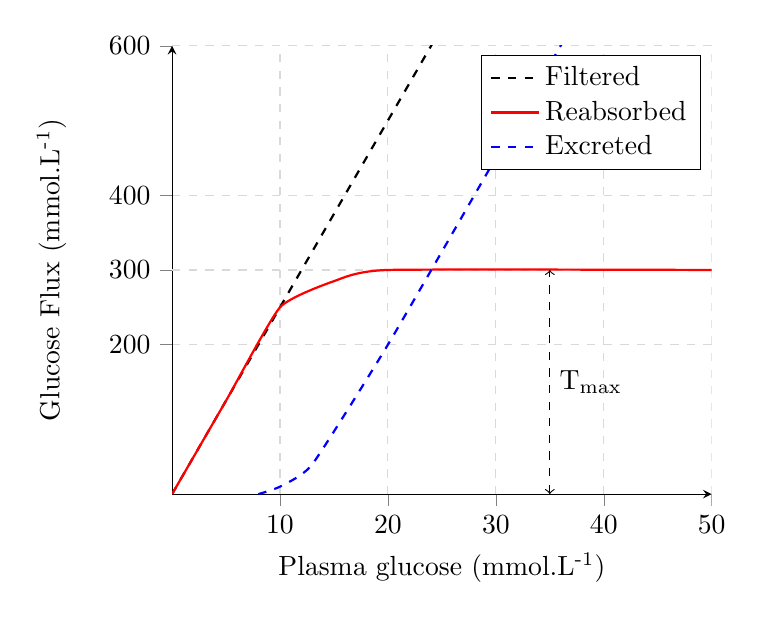
\begin{tikzpicture}[dot/.style={circle,inner sep=1pt,fill,label={#1},name=#1},
 extended line/.style={shorten >=-#1,shorten <=-#1},
 extended line/.default=10cm]

    \begin{axis}[
        axis x line=middle,
        axis y line=middle,
        grid = major,
        grid style={dashed, gray!30},
    	  x label style={at={(axis description cs:0.5,-0.1)},anchor=north},
	  y label style={at={(axis description cs:-0.1,.5)},rotate=90,anchor=south},
        xmin=0,
        xmax= 50,
        ymin= 0,
        ymax= 600,
	extra y ticks={300},
	 ylabel near ticks,
	xlabel near ticks,
        xlabel=Plasma glucose (mmol.L\textsuperscript{-1}),
        ylabel=Glucose Flux (mmol.L\textsuperscript{-1}),
        tick align=outside,
        enlargelimits=false,
legend cell align={left}]

\addplot[domain=0:50, black, dashed, thick] {25*x};
\addlegendentry{Filtered}

\draw[red, thick] plot[smooth,tension=0.3] coordinates { (axis cs: 0,0) (axis cs: 5,125)  (axis cs: 10, 250) (axis cs: 15,285) (axis cs: 20,300) (axis cs: 50,300)};

\draw[blue, thick,dashed] plot[smooth,tension=0.3] coordinates {(axis cs: 8,0) (axis cs: 10,10) (axis cs: 13,40) (axis cs: 20,200) (axis cs: 30,450) (axis cs: 40,700)};

\draw[black,thin,dashed,<->] (axis cs: 35,0) -- node[black,right]{T\textsubscript{max}} (axis cs: 35,300);

\addlegendimage{red, thick};
\addlegendentry{Reabsorbed};
\addlegendimage{blue,dashed,thick};
\addlegendentry{Excreted};

\end{axis}


\end{tikzpicture} 
\end{document}